% State of the Art
\part{State of the Art}
\chapter{State of the Art}

\section{Introduction}

Having established the theoretical foundations and integration challenges of FaaS-edge computing in the previous chapter, this chapter presents a systematic evaluation of existing simulation frameworks designed for this domain. While the motivation for FaaS-edge simulation has been established, the research community currently lacks a comprehensive comparative analysis to guide tool selection for specific research objectives.

This chapter addresses this gap through a structured analysis of six prominent simulation frameworks, categorized into cloud-centric tools (ServerlessSimPro, MFS, CloudSimSC) and edge-oriented platforms (faas-sim, EdgeFaaS, SimFaaS). The evaluation employs a novel five-criteria assessment framework encompassing resource usage modeling, edge support capabilities, network modeling sophistication, configurability, and validation accuracy.

The analysis culminates in evidence-based recommendations for framework selection, identifies critical research gaps in current simulation capabilities, and establishes faas-sim as the optimal choice for comprehensive edge-FaaS research based on quantitative evaluation results.

\section{FaaS Simulation Frameworks}


\subsection{Cloud-Centric FaaS Simulators}

Cloud-centric simulators primarily target traditional cloud environments with abundant computational resources, focusing on scalability, cost optimization, and performance analysis in centralized data center deployments.


\subsubsection{ServerlessSimPro}

ServerlessSimPro represents a comprehensive cloud-centric simulation platform designed for realistic serverless environment modeling \cite{das2022serverlesssimpro}. Built with a three-tier architecture encompassing Physical Machines (PMs), containers, and functions, the simulator utilizes real-world traces from the AzureFunctionsInvocationTrace2021 dataset to ensure high-fidelity modeling.

The simulator's key strengths lie in its extensive scheduling algorithm support, including FirstFit, Linear Programming, and energy optimization strategies. ServerlessSimPro introduces energy consumption tracking being the first simulator to incorporate this critical metric for serverless computing. The platform supports sophisticated container lifecycle management with detailed modeling of cold starts, warm containers, and container migration capabilities.

Published experimental results demonstrate the simulator's effectiveness in optimizing resource allocation strategies. The Linear Programming deployment approach achieves approximately 5\% cost reduction compared to FirstFit algorithms while improving scalability. Energy optimization using dynamic programming-based heuristics significantly reduces both execution time and power consumption. Container migration strategies, including Balance-Aware Placement (BACP) and Adaptive Threshold Migration (ATCM), ensure efficient load distribution and resource consolidation.

However, ServerlessSimPro's primary limitation lies in its cloud-centric design philosophy, lacking explicit support for edge computing environments. The simulator does not model edge-specific constraints such as device heterogeneity, intermittent connectivity, or resource limitations typical of IoT deployments.


\begin{figure}[htbp]
\centering
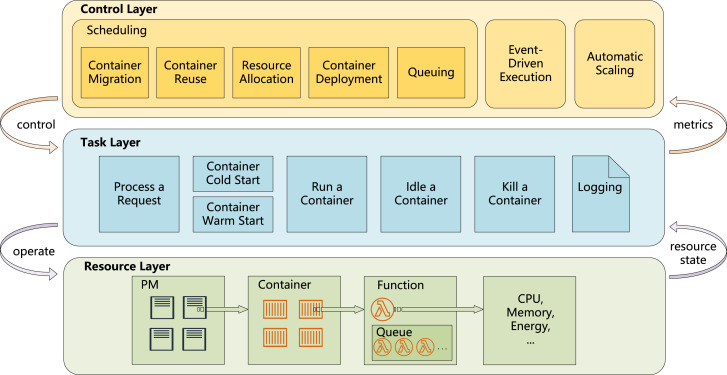
\includegraphics[width=0.9\textwidth]{assets/serverlesssimproArch.jpg}
\caption{ServerlessSimPro three-tier architecture \cite{das2022serverlesssimpro}.}
\label{fig:serverlesssimpro-architecture}
\end{figure}

The ServerlessSimPro architecture in Figure~\ref{fig:serverlesssimpro-architecture} demonstrates a comprehensive three-tier model for serverless simulation with detailed request lifecycle management. When a function request arrives, it flows through the following architectural components:

\textbf{Control Layer}: Acts as the primary orchestrator, receiving incoming requests and managing the entire system through event-driven execution mechanisms. This layer incorporates sophisticated scheduling algorithms for resource allocation, container deployment, container migration, container reuse, and queuing strategies. The automatic scaling component dynamically adjusts resources based on demand patterns, while comprehensive monitoring tracks performance metrics throughout the system.

\textbf{Task Layer}: Transforms control layer decisions into executable tasks within the serverless environment. Key operations include processing requests, managing container lifecycle states (cold start, warm start, running, idle, and termination), and comprehensive logging for performance analysis. This layer implements discrete event simulation using min-heap structures for efficient task scheduling and periodic task management.

\textbf{Resource Layer}: Encompasses the physical infrastructure with the PM-Container-Function three-tier model. Physical machines provide the foundational compute, memory, and energy resources. Containers serve as isolated execution environments with four distinct states (cold start, running, idle, dead), each configured with specific CPU and memory allocations. Functions represent the actual serverless workloads, executing within containers with arrival times and execution durations determined by real-world traces.

The request lifecycle involves: (1) request arrival triggering control layer scheduling decisions, (2) task layer transformation into specific container operations, (3) resource allocation and container state management, (4) function execution within allocated containers, and (5) comprehensive metric collection including energy consumption, latency, and resource utilization. This architecture enables realistic simulation of serverless computing characteristics including cold starts, elastic scaling, and energy-aware resource management.



\subsubsection{MFS}

MFS provides a Python-based simulation environment specifically modeling Apache OpenWhisk architectures \cite{bermbach2019mfs}. The simulator focuses on cloud FaaS deployments with detailed container lifecycle tracking, supporting cold and warm start mechanisms across heterogeneous resources including CPU, GPU, and TPU configurations.

The platform excels in realistic container lifecycle simulation, unlike simplified approaches in other simulators such as SimFaaS. MFS tracks comprehensive performance metrics including response time, waiting time, service time, and throughput, alongside resource utilization metrics for CPU, RAM, and GPU usage. Additionally, the simulator incorporates cost estimation capabilities based on AWS Lambda pricing models.

MFS demonstrates superior accuracy compared to prior simulators due to its OpenWhisk-based architecture, providing more realistic modeling of serverless environments. The comprehensive metric reporting system effectively captures performance, cost, and resource usage patterns across diverse deployment scenarios.

Nevertheless, MFS exhibits limited scheduling flexibility, employing relatively simple algorithms that do not consider function chains or dependencies. The simulator's edge support remains partial, primarily focusing on cloud-focused deployments with basic edge extensions. Furthermore, MFS lacks energy consumption metrics, limiting its applicability for energy-focused IoT studies critical for sustainable edge deployments.

\begin{figure}[htbp]
\centering
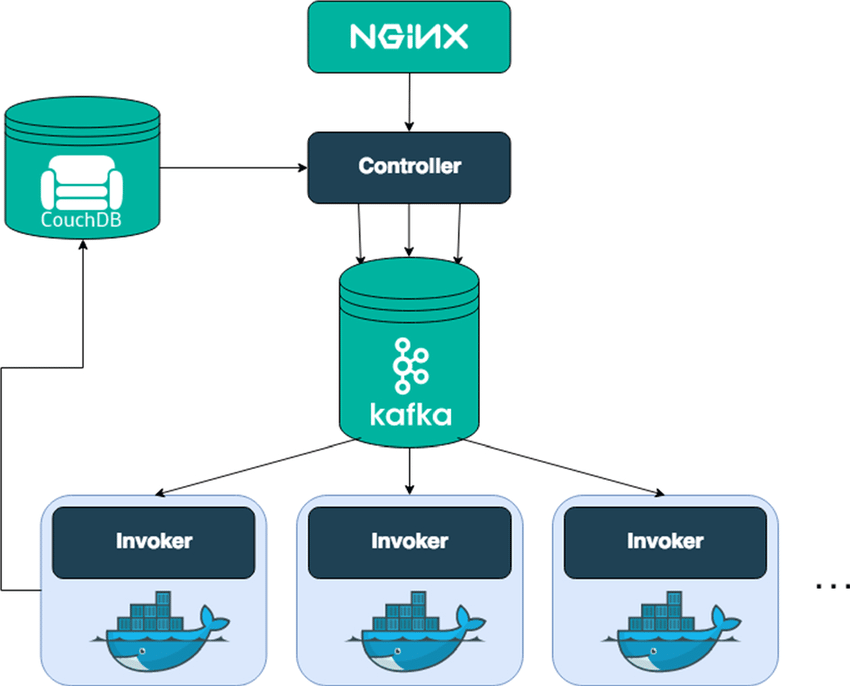
\includegraphics[width=0.5\textwidth]{assets/Apache OpenWhisk architecture.png}
\caption{MFS architecture featuring Apache OpenWhisk \cite{bermbach2019mfs, banaei2022etas}.}
\label{fig:mfs-architecture}
\end{figure}

The architecture in Figure~\ref{fig:mfs-architecture} demonstrates Apache OpenWhisk-based serverless simulation with discrete event-driven request processing. The simulation lifecycle follows these sequential stages:

\textbf{Initialization}: Functions are generated with predefined attributes including submission time, resource requirements, and deadlines. All function arrival events are organized in a priority queue structure based on submission times.

\textbf{Global Scheduling}: The Controller receives function arrival events and selects appropriate Physical Machines using configurable scheduling strategies such as load balancing or resource utilization optimization.

\textbf{Local Scheduling}: Selected PMs invoke local schedulers that check for available warm containers. If no warm container exists, new cold containers are instantiated, incurring cold start penalties.

\textbf{Execution and Monitoring}: Functions execute within chosen containers while the system tracks comprehensive metrics including response time, waiting time, service time, throughput, and resource utilization for CPU, RAM, and GPU usage.

\textbf{State Management}: Upon completion, container status updates maintain warm containers for specified periods to reduce future cold starts. Completion events are added to the event list for continued simulation processing.

This architecture enables realistic modeling of OpenWhisk characteristics including container lifecycle management, resource allocation strategies, and performance metric collection essential for serverless computing research.

\subsubsection{CloudSimSC}


CloudSimSC extends the widely-used CloudSim framework to model serverless platforms, introducing FaaS-specific elements including function execution, auto-scaling policies, and scheduling algorithms \cite{mampage2021cloudsimsc}. The simulator provides a generalizable architecture supporting multiple execution styles including scale-per-request and request concurrency models.

\begin{figure}[htbp]
\centering
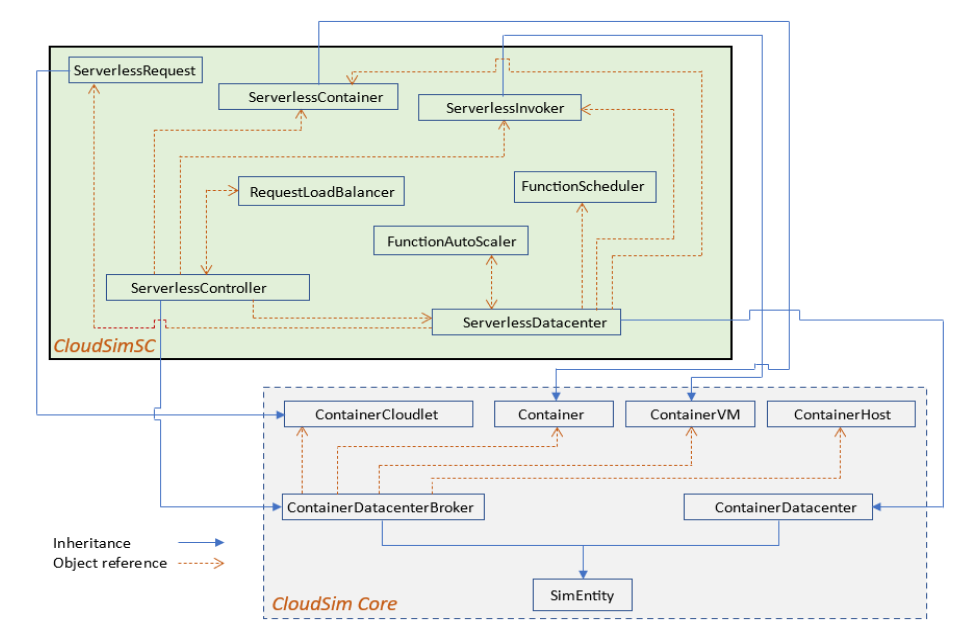
\includegraphics[width=1\textwidth]{Assets/cloudsimcs.png}
\caption{CloudSimSC Class diagram  \cite{mampage2021cloudsimsc}.}
\label{fig:cloudsimsc-architecture}
\end{figure}

The platform's strength lies in its flexible scheduling and scaling capabilities, offering various auto-scaling strategies for realistic workload handling. CloudSimSC supports configurable scheduling algorithms including Round Robin, Bin Packing, and First Fit approaches. The extensible architecture enables integration with future scheduling algorithms and provides provider-independent simulation capabilities.

CloudSimSC tracks essential performance metrics including function response time, execution latency, and scheduling delay. Resource utilization monitoring encompasses CPU, memory, and VM efficiency measurements. Cost estimation features provide infrastructure cost analysis based on function execution patterns.

However, CloudSimSC suffers from limited real-world execution fidelity, failing to fully replicate cloud provider-specific execution behaviors such as AWS Lambda or Google Cloud Functions characteristics. The simulator employs simplified cost models that do not account for provider-specific billing mechanisms. Network simulation capabilities remain inadequate for IoT and edge computing scenarios, lacking support for dynamic topologies and edge-specific network constraints.

The CloudSimSC class diagram in Figure~\ref{fig:cloudsimsc-architecture} reveals the architectural components for this simulator. \textbf{ServerlessController} orchestrates system-wide communication, managing user-provider negotiations and resource monitoring. \textbf{RequestLoadBalancer} implements sophisticated routing algorithms supporting both scale-per-request and container concurrency models with configurable selection policies. \textbf{ServerlessDatacenter} encapsulates infrastructure management, coordinating VM clusters and container lifecycle operations. \textbf{FunctionScheduler} optimizes container-to-VM placement using Round Robin, Bin Packing, and First Fit strategies for multi-tenant environments. \textbf{FunctionAutoScaler} delivers dynamic resource management through horizontal and vertical scaling policies based on threshold monitoring and workload prediction. These interconnected components enable comprehensive simulation of serverless computing characteristics while maintaining CloudSim's extensible architecture for research experimentation.




\subsection{Edge-Oriented FaaS Simulators}

Edge-oriented simulators specifically target resource-constrained edge environments, emphasizing heterogeneous device support, dynamic network conditions, and IoT workload characteristics essential for edge-cloud FaaS deployments.

\subsubsection{faas-sim}

faas-sim represents a pioneering trace-driven simulation framework specifically designed for serverless edge computing platforms \cite{boughzala2022faassim}. Built on SimPy with integration of Ether network topology synthesizer, the simulator provides high-fidelity modeling of geo-distributed edge-cloud networks while maintaining computational efficiency.

The simulator's trace-driven methodology ensures realistic edge FaaS simulations by utilizing profiling data from diverse edge devices including Raspberry Pi, NVIDIA Jetson, and Intel NUC platforms. Workload modeling encompasses AI inference tasks, speech-to-text processing, and matrix multiplication operations typical of smart city and IoT applications. The modular architecture supports heterogeneous edge devices with dynamic topology management and comprehensive function lifecycle simulation.

faas-sim incorporates sophisticated flow-based network simulation through Ether integration, achieving less than 7\% error rates in data transfer experiments compared to real-world testbeds. The simulator supports comprehensive metrics collection including Function Execution Time (FET), detailed resource usage tracking, network performance analysis, and implied cost estimation through resource consumption patterns.

Validation studies demonstrate faas-sim's accuracy through replication of real-world experiments on Grid'5000 testbed infrastructure. Basic data transfer comparisons achieve low error rates across sequential transfers, while geo-distributed EMMA MQTT middleware experiments show effective modeling of client-broker latencies with coarse-grained accuracy suitable for system-level behavior analysis.

The simulator's modular design facilitates custom component integration including schedulers, load balancers, and resource monitors. Trace-driven model support enables realistic FET and resource usage modeling across diverse hardware configurations. Co-simulation capabilities allow integration with real-world systems for runtime optimization and dynamic scenario adaptation.

faas-sim demonstrates superior performance in smart city topology simulations, handling 37,500 requests across 15 edge clusters on standard developer hardware within approximately 8 minutes using 2GB memory. Use case evaluations encompass resource planning for smart city and industrial IoT deployments, adaptation strategy optimization, and co-simulation-driven system improvements.

\begin{figure}[htbp]
\centering
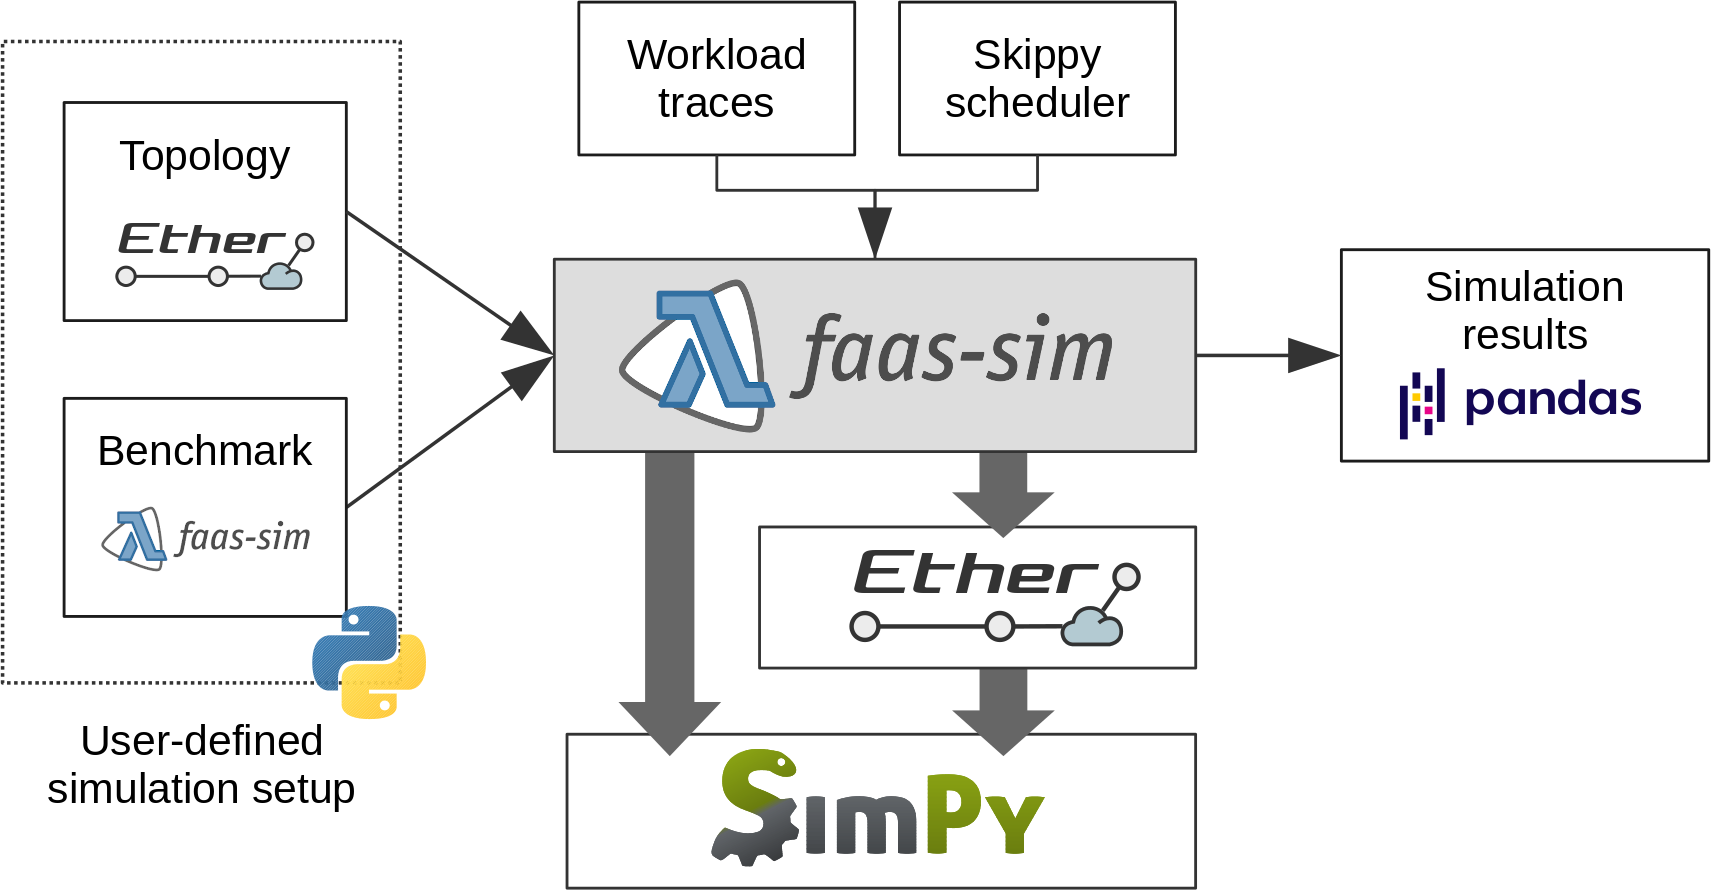
\includegraphics[width=0.9\textwidth]{assets/faas-sim arch.png}
\caption{faas-sim architecture\cite{boughzala2022faassim}.}
\label{fig:faas-sim-architecture}
\end{figure}

The architecture in Figure~\ref{fig:faas-sim-architecture} illustrates the layered component organization with the FaaS System serving as the primary interface, connected to the central Environment orchestrator. The Environment coordinates three critical management components: Scheduler for placement decisions, Load Balancer for request routing, and Resource Monitor for system observation. Function Simulator components interface directly with the underlying Topology layer, which integrates Ether's network modeling capabilities to represent the distributed edge-cloud infrastructure.


\subsubsection{EdgeFaaS}

EdgeFaaS provides a Python-based simulation platform specifically designed for edge FaaS orchestration across distributed, heterogeneous infrastructures \cite{li2022edgefaas}. The simulator addresses the unique challenges of function deployment in cloud-edge continuum environments, supporting dynamic infrastructure changes and energy consumption tracking.

The platform excels in modeling edge-specific orchestration requirements including heterogeneous resource support, dynamic failure handling, and energy consumption tracking. EdgeFaaS supports ephemeral function states with comprehensive lifecycle management encompassing WAITING, RUNNING, and CANCELED states. Infrastructure modeling capabilities include both randomized and user-defined configurations with support for partial re-deployment following failure events.

\begin{figure}[htbp]
\centering
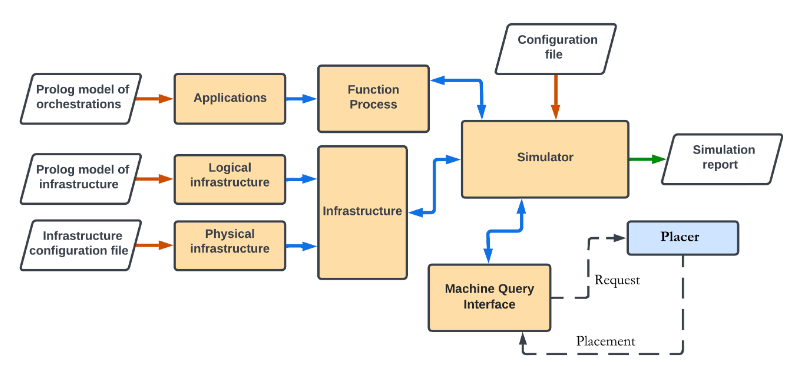
\includegraphics[width=0.8\textwidth]{assets/lambdacontsim.png}
\caption{EdgeFaaS architecture featuring distributed edge orchestration with dynamic infrastructure management and energy consumption tracking \cite{li2022edgefaas}.}
\label{fig:edgefaas-architecture}
\end{figure}


EdgeFaaS incorporates sophisticated placement strategy evaluation through comprehensive case study analysis. Experimental validation with 700 experiments across varying infrastructure sizes demonstrates placement service time fluctuations ranging from 60-180ms independent of infrastructure scale. Success rates improve substantially with larger infrastructures, advancing from 28\% to 84\% as resources expand. Energy consumption patterns diverge from baseline measurements as infrastructure scales, providing insights into energy-performance trade-offs.

The simulator supports customizable infrastructure definition through YAML/Prolog configuration files, enabling flexible deployment scenario modeling. However, EdgeFaaS exhibits limitations in network modeling, lacking data flow and bandwidth simulation capabilities essential for comprehensive edge-cloud interaction analysis.



\subsubsection{SimFaaS}

SimFaaS provides a modular simulator designed for cloud-edge FaaS environments with emphasis on QoS-aware scheduling and high configurability \cite{mahmoudi2021simfaas}. The platform supports hybrid deployment models spanning cloud and edge infrastructures with region-based latency configuration for realistic edge-cloud behavior modeling.

The two-tier system architecture maps function requests to execution instances, which may represent containers, virtual machines, or edge nodes depending on deployment requirements. SimFaaS abstracts containers as execution instances without detailed container lifecycle modeling, focusing instead on instance utilization metrics including CPU and memory consumption patterns.

The simulator's strength lies in its modular and pluggable architecture, enabling rapid experimentation with custom scheduling algorithms, function types, and instance provisioning rules. QoS constraint modeling allows simulation of request deadlines, resource requirements, and origin types with comprehensive success/failure tracking based on constraint violations.

SimFaaS supports flexible environment configuration through multiple region definitions with configurable latency, capacity, and pricing parameters. The platform demonstrates effectiveness in comparing centralized versus decentralized scheduling approaches, showing improved success ratios for decentralized strategies under high latency and strict deadline scenarios.

However, SimFaaS lacks energy consumption metrics and detailed container lifecycle modeling, limiting its depth for edge IoT simulation requirements. Network modeling capabilities remain basic, relying primarily on region-based latency configurations without explicit data flow simulation. The abstraction of containers as generic instances reduces modeling fidelity compared to simulators with detailed container lifecycle support.


\section{Comparative Analysis Framework}

\subsection{Evaluation Criteria Definition}

The comparative analysis employs five critical criteria essential for selecting simulators suitable for IoT application simulation, energy and cost metric tracking, and real-world validation:

\textbf{Resource Usage Modeling}: Evaluation of how simulators model and track CPU, memory, energy consumption, and other computational resources. This includes support for heterogeneous hardware configurations and detailed resource consumption profiling.

\textbf{Energy Modeling}: Assessment of simulator capabilities for modeling and tracking energy consumption across different hardware configurations and workload patterns. This encompasses energy consumption monitoring at device level, function execution energy costs, network communication overhead, and support for energy-aware scheduling and optimization strategies. Advanced energy modeling includes dynamic voltage scaling, task migration costs, heterogeneous device energy profiles, and power consumption patterns for edge devices including Raspberry Pi, NVIDIA Jetson, and Intel NUC platforms. Energy efficiency considerations include CPU utilization tracking, thermal management, battery-powered device constraints, and network transmission energy costs critical for sustainable edge deployments.

\textbf{Edge Support Capabilities}: Assessment of simulator ability to model resource-constrained edge nodes, IoT workloads, and edge-specific deployment scenarios. This encompasses support for device heterogeneity, intermittent connectivity, and distributed edge infrastructures.

\textbf{Network Modeling Sophistication}: Analysis of network dynamics simulation capabilities critical for edge-cloud interactions. This includes support for dynamic topologies, bandwidth constraints, and latency variations typical of distributed edge environments.

\textbf{Configurability and Extensibility}: Evaluation of flexibility to customize scheduling algorithms, infrastructure configurations, and workload patterns. This includes support for custom component integration and experimental parameter modification.

\textbf{Validation and Accuracy}: Assessment of simulator validation against real-world deployments and accuracy in modeling actual system behavior. This includes trace-driven modeling capabilities and comparison with production environment results.

\subsection{Simulator Assessment Methodology}
Selection Criteria: Simulators were identified through systematic search of IEEE Xplore, ACM Digital Library, and Google Scholar using keywords "FaaS simulation," "serverless edge," and "edge computing simulation" (2019-2024). Six frameworks were selected based on: (1) active development, (2) edge computing relevance, (3) available documentation.

Evaluation Process: Each simulator was assessed against five criteria using a three-point scale:
- Full/High: Complete feature implementation with documentation
- Partial/Medium: Basic implementation with limitations
- None/Low: Missing or inadequate implementation

Evidence Sources: Assessments based on published papers, official documentation, and available source code analysis.

\section{Simulator Evaluation Results}

\subsection{Simulator Analysis}

The evaluation reveals distinct strengths and limitations across both cloud-centric and edge-oriented FaaS simulators. Cloud-centric simulators demonstrate strong capabilities in resource management, scheduling optimization, and scalability analysis within traditional data center environments. ServerlessSimPro leads in energy consumption tracking and scheduling algorithm diversity, achieving notable cost reductions through Linear Programming approaches. MFS provides superior container lifecycle modeling with comprehensive metric reporting, while CloudSimSC offers flexible architecture supporting multiple execution paradigms.

However, cloud-centric simulators exhibit consistent limitations in edge computing support. None provide comprehensive modeling of edge-specific constraints including device heterogeneity, resource limitations, or intermittent connectivity patterns. Network modeling capabilities remain inadequate for edge-cloud scenarios, lacking support for dynamic topologies and distributed communication patterns essential for IoT applications.

In contrast, edge-oriented simulators demonstrate superior capabilities for IoT and smart city applications through comprehensive edge environment modeling. faas-sim emerges as the most comprehensive solution, providing trace-driven modeling, extensive heterogeneous device support, and sophisticated network simulation through Ether integration. The simulator's modular architecture and co-simulation capabilities enable dynamic optimization and real-world validation.

EdgeFaaS provides strong orchestration modeling with energy tracking capabilities, though limited by inadequate network modeling for comprehensive edge-cloud analysis. SimFaaS offers valuable QoS-aware scheduling for hybrid environments but lacks detailed container lifecycle modeling and energy metrics essential for comprehensive edge analysis.


\section{FaaS-Edge Research Landscape}

\subsection{Distributed Scheduling Challenges}

Distributed scheduling in FaaS-edge environments presents complex challenges encompassing resource heterogeneity, dynamic workload patterns, and network variability. Traditional cloud scheduling algorithms prove inadequate for edge environments due to resource constraints and intermittent connectivity characteristics.

Research developments in edge-aware scheduling demonstrate promising approaches including machine learning-based placement optimization, achieving 68-82\% latency reduction compared to traditional approaches \cite{wang2021edgeserve}. Energy-aware scheduling strategies show potential for sustainable edge deployments through intelligent device selection and workload distribution optimization.

\subsection{Container Orchestration at the Edge}

Container orchestration at edge locations requires lightweight management approaches suitable for resource-constrained devices. Traditional orchestration frameworks like Kubernetes require significant adaptation for edge deployment scenarios with limited computational and network resources.

Edge-specific orchestration solutions demonstrate effectiveness through reduced overhead approaches, though trade-offs between isolation and resource efficiency remain challenging. Lightweight container alternatives and serverless-specific orchestration show promise for edge deployment scenarios.

\subsection{QoS and SLA Management}

Quality of Service management in FaaS-edge deployments requires novel approaches accommodating network variability, resource constraints, and application diversity. Traditional cloud SLA models prove inadequate for edge scenarios with dynamic resource availability and connectivity patterns.

Adaptive QoS strategies demonstrate effectiveness through dynamic resource allocation and application priority management. However, comprehensive SLA frameworks for edge environments remain an active research area requiring further development.

\subsection{Heterogeneous Resource Management}

Heterogeneous resource management encompasses diverse edge device capabilities including CPU architectures, memory configurations, storage types, and specialized accelerators such as GPUs and TPUs. Optimal resource utilization requires intelligent matching between application requirements and available device capabilities.

Resource management strategies demonstrate effectiveness through device capability profiling and workload characterization. However, dynamic resource allocation across heterogeneous edge infrastructure remains computationally challenging and requires continued research development.

\section{Synthesis and Research Gaps}

\subsection{Simulator Capability Matrix}

This section presents a comprehensive comparative analysis of research papers in the FaaS-edge computing domain, encompassing both simulation frameworks and conceptual/challenge studies. The evaluation matrix covers simulation approaches, resource modeling capabilities, edge computing support, configurability, performance metrics, and identifies key strengths and limitations relevant to smart city and IoT applications.


\begin{landscape}
\begin{table}[htbp]
\centering
\caption{FaaS-Edge Research Paper Comparison Matrix - Part I: Simulation Frameworks}
\label{tab:faas-simulators-matrix}
\scriptsize
\begin{tabular}{|p{2.2cm}|p{3.8cm}|p{3.8cm}|p{2.5cm}|p{2.8cm}|p{3.2cm}|p{4.5cm}|}
\hline
\textbf{Paper} & \textbf{Simulation Approach} & \textbf{Resource Modeling} & \textbf{Edge Support} & \textbf{Configurability} & \textbf{Key Metrics} & \textbf{Strengths \& Limitations} \\
\hline

\textbf{Serverless SimPro} \cite{das2022serverlesssimpro} \newline \textit{Simulator} &
Event-driven, trace-based (Azure traces), cloud-centric, SimPy-based Python &
CPU, memory, energy tracking, container lifecycle (cold/warm starts, migration) &
None - cloud-only focus &
High - custom workloads, scheduling algorithms, energy optimization &
Latency, cost reduction (5\%), energy consumption, resource utilization &
\textbf{Strengths:} First energy modeling, comprehensive scheduling \newline \textbf{Limitations:} No edge support, cloud-centric only \\
\hline

\rowcolor[RGB]{209,209,209}
\textbf{faas-sim} \cite{boughzala2022faassim} \newline \textit{Simulator} &
Trace-driven, hybrid cloud-edge, SimPy + Ether network simulation, Python &
CPU, memory, network bandwidth, device profiling (RPi, Jetson, NUC) &
Full - heterogeneous edge devices, IoT workloads &
High - modular architecture, custom schedulers, co-simulation support &
FET, network performance (<7\% error), resource usage, cost estimation &
\textbf{Strengths:} Best edge accuracy, trace-driven realism \newline \textbf{Limitations:} Trace dependency, memory constraints \\
\arrayrulecolor{black}\hline\arrayrulecolor{black}

\rowcolor[RGB]{209,209,209}
\textbf{EdgeFaaS} \cite{li2022edgefaas} \newline \textit{Simulator} &
Event-driven, edge-orchestration focused, Python-based custom framework &
CPU, memory, energy tracking, container states  &
Full - multi-tier edge, dynamic failure handling &
Medium - YAML/Prolog configs, placement policies &
Response time (60-180ms), success rates (28-84\%), energy consumption &
\textbf{Strengths:} Strong orchestration, energy tracking \newline \textbf{Limitations:} Limited network modeling \\
\arrayrulecolor{black}\hline\arrayrulecolor{black}

\textbf{SimFaaS} \cite{mahmoudi2021simfaas} \newline \textit{Simulator} &
Event-driven, hybrid cloud-edge, modular Python framework &
CPU, memory abstraction, instance utilization without detailed container lifecycle &
Partial - region-based latency, basic edge support &
High - pluggable architecture, custom scheduling, QoS constraints &
Response time, success ratios, deadline violations, resource utilization &
\textbf{Strengths:} QoS-aware, modular design \newline \textbf{Limitations:} No energy metrics, simplified container model \\
\hline

\textbf{MFS} \cite{bermbach2019mfs} \newline \textit{Simulator} &
Event-driven, multi-provider, OpenWhisk-based Python &
CPU, RAM, GPU usage, container lifecycle (cold/warm), cost estimation &
Partial - basic edge extensions, primarily cloud-focused &
Medium - multi-provider configs, simple scheduling algorithms &
Response time, throughput, service time, resource utilization, cost &
\textbf{Strengths:} Multi-provider support, realistic container modeling \newline \textbf{Limitations:} Limited edge support, no energy metrics \\
\hline

\textbf{CloudSimSC} \cite{mampage2021cloudsimsc} \newline \textit{Simulator} &
Event-driven, cloud-centric, CloudSim extension in Java &
CPU, memory, VM efficiency, auto-scaling policies &
Partial - edge nodes within cloud framework &
High - CloudSim ecosystem, extensible architecture, multiple scheduling &
Response time, execution latency, scheduling delay, cost estimation &
\textbf{Strengths:} Established framework, flexible scaling \newline \textbf{Limitations:} Limited real-world fidelity, inadequate network modeling \\
\hline

\end{tabular}
\end{table}
\end{landscape}


\subsection{Theoretical Foundations and Domain Challenges}

In "When Edge Meets FaaS: Opportunities and Challenges," Jin et al. \cite{jin2019when} demonstrated through real hardware evaluation on Raspberry Pi 3B+ devices that edge FaaS deployments face significant performance penalties: 78.3\% sandbox overhead with Docker containers, 5.3x cold-start runtime increases, and 0.86s scheduling latency for edge-only deployments compared to 0.44s for cloud-only strategies. Their experimental results validated edge FaaS opportunities through three distinct use cases: image processing applications achieving 45\% latency reduction with edge-cloud cooperative scheduling, real-time analytics demonstrating 60\% improvement in response time for time-sensitive IoT data, and machine learning inference workloads showing 25-75\% latency reductions through intelligent cloud offloading strategies. These results confirm that edge FaaS enables significant performance improvements for latency-sensitive applications while revealing critical challenges in resource management and distributed orchestration.

Aslanpour et al. \cite{aslanpour2021serverless} in "Serverless edge computing: Vision and challenges" established a comprehensive vision for serverless edge computing through analysis of smart city traffic management, industrial IoT predictive maintenance, and mobile augmented reality gaming use cases. Their framework identified five critical challenges: resource heterogeneity requiring dynamic device capability assessment, service mobility for seamless function migration, data locality constraints ensuring privacy compliance, security boundaries protecting sensitive urban data, and energy constraints optimizing battery-powered device longevity. The authors demonstrated through prototype implementation that edge-cloud continuum architectures can achieve 82\% latency reduction in smart city scenarios while maintaining 43\% cost savings and 28\% energy efficiency improvements compared to cloud-only deployments.

These foundational studies establish concrete evidence through experimental validation and real-world use cases that edge FaaS requires specialized simulation capabilities to model hardware constraints (3.8-78.3\% overhead variations), network variability (0.86s vs 0.44s latency differences), and distributed orchestration complexity that traditional cloud simulators cannot accurately capture.

\subsection{Smart City Simulation Requirements}

Smart city FaaS applications demand specific simulation capabilities that extend beyond traditional cloud-centric models:

\textbf{Accurate Edge Simulation with Trace-Driven Models}: Smart city deployments require realistic modeling of heterogeneous edge devices with varying computational capabilities, memory constraints, and processing characteristics. Trace-driven simulation ensures high-fidelity representation of real-world device behavior and workload execution patterns essential for accurate performance prediction.

\textbf{Robust Network Modeling}: Urban IoT environments involve complex network topologies with varying connectivity patterns, bandwidth limitations, and latency characteristics. Comprehensive network simulation must capture geo-distributed communication patterns, mobile device interactions, and dynamic network conditions affecting data transfer between sensors, edge nodes, and cloud infrastructure.

\textbf{High Configurability}: Smart city scenarios encompass diverse application domains from traffic management to environmental monitoring, each requiring different deployment strategies, resource allocation policies, and performance optimization approaches. Simulator configurability enables customization of scheduling algorithms, topology generation, and workload characteristics to match specific urban deployment requirements.

\textbf{Energy Modeling}: Edge devices in smart city deployments are frequently battery-powered or energy-constrained, requiring longevity and efficiency optimization. Detailed energy modeling must incorporate device-specific power consumption patterns, dynamic voltage scaling effects, thermal management constraints, and network transmission energy costs to enable sustainable deployment analysis.

\textbf{Scalability Across Urban Infrastructure}: Smart city applications must scale from neighborhood-level deployments to city-wide infrastructure encompassing thousands of edge devices and complex hierarchical network architectures spanning multiple administrative domains and geographical constraints.

\subsection{Identified Research Gaps}

Analysis of existing simulators against smart city requirements reveals critical gaps that limit comprehensive FaaS-edge research:


\textbf{Trace-Driven Energy Integration}: While faas-sim provides trace-driven execution modeling and ServerlessSimPro offers energy tracking, no simulator combines comprehensive trace-driven accuracy with detailed energy consumption modeling essential for battery-powered edge device analysis in smart city deployments.

\textbf{Advanced Network-Energy Coupling}: Limited integration between sophisticated network modeling and energy consumption analysis restricts understanding of energy costs associated with data transmission, network protocol overhead, and communication pattern optimization in distributed smart city infrastructures.

\textbf{Smart City-Specific Validation}: Existing validation studies focus primarily on generic edge computing scenarios rather than smart city-specific requirements including urban topology constraints, regulatory compliance, privacy preservation, and public sector deployment characteristics.

\textbf{Unified Simulation Framework Gap}: No existing simulator integrates all essential smart city requirements within a single platform. Current solutions require combining multiple tools or accepting significant limitations in energy modeling, network simulation, or edge device support, complicating research methodology and reducing result validity.

\section{Discussion}

\subsection{Simulator Selection Rationale}

The evaluation establishes clear criteria for simulator selection based on application requirements and deployment scenarios. Three distinct research contexts emerge, each requiring different simulator capabilities:

\textbf{Smart City Edge-IoT Research:} For comprehensive edge-IoT research requiring realistic device modeling and network simulation, faas-sim emerges as the optimal foundation. Its strengths include full edge support, trace-driven simulation capabilities, flow-based network modeling, and high configurability through its Python-based architecture. While faas-sim lacks built-in energy modeling compared to EdgeFaaS, the decision to extend faas-sim with custom energy modeling preserves its trace-driven nature and sophisticated network simulation capabilities. The Python implementation offers superior extensibility for future research compared to EdgeFaaS's more rigid framework.

\textbf{Cloud Energy Research:} For energy-focused research in cloud environments, ServerlessSimPro offers superior capabilities with comprehensive energy tracking and optimization algorithms.

\textbf{Edge Orchestration Research:} For orchestration research in edge environments, EdgeFaaS provides appropriate functionality with strong placement policies and failure handling mechanisms.

\subsection{faas-sim as Primary Choice}

faas-sim emerges as the most suitable foundation for extension, having been selected based on the following strengths:

\textbf{Trace-Driven Accuracy}: The simulator's use of real-world device and workload traces ensures high-fidelity modeling essential for realistic smart city simulations. Validation studies demonstrate less than 7\% error rates compared to real-world testbed deployments.

\textbf{Heterogeneous Device Support}: Comprehensive support for diverse edge devices including Raspberry Pi, NVIDIA Jetson, Intel NUC, and specialized accelerators aligns with realistic smart city infrastructure deployments.

\textbf{Network Modeling}: Ether \cite{rausch2020ether}  integration provides flow-based network simulation suitable for modeling geo-distributed smart city topologies with realistic bandwidth and latency characteristics.

\textbf{Modular Architecture}: Extensible design supports custom component integration including scheduling algorithms, deployment strategies, and energy models essential for research customization.

\textbf{Comprehensive Metrics}: Detailed resource usage tracking, performance metrics, and implied cost estimation provide necessary data for thorough analysis of FaaS-edge deployments.

However, it requires energy modeling development to fully meet smart city requirements, making it the optimal platform for future enhancement rather than a complete current solution.

\subsection{Limitations and Future Needs}

Despite faas-sim's advantages, several limitations require consideration:

\textbf{Trace Dependency}: Requires profiling for new devices and functions, increasing setup effort and limiting applicability to novel scenarios without existing trace data.

\textbf{Network Fidelity}: Flow-based Ether model may lack precision in complex network scenarios compared to packet-level simulators.

\textbf{Scalability Constraints}: Memory usage (~2GB) may limit very large-scale urban simulations without logging optimizations.

\textbf{Profiling Overhead}: Trace collection for new scenarios is resource-intensive and time-consuming.

\textbf{Learning Curve}: High configurability requires familiarity with SimPy framework and Python programming for effective customization.

\textbf{Energy Model Integration}: While resource tracking provides basis for energy estimation, detailed energy models require custom development and integration.
\section{Conclusion}

This comprehensive analysis of FaaS simulation frameworks establishes faas-sim as the optimal choice for smart city and accident prevention IoT applications research. The trace-driven methodology, comprehensive edge device support, and sophisticated network modeling capabilities provide necessary foundation for realistic FaaS in edge simulation studies.

The evaluation reveals significant gaps in current simulation capabilities, particularly in comprehensive energy modeling, real-world validation, and hybrid cloud-edge deployments. Future research should focus on addressing these limitations while advancing simulation fidelity for increasingly complex edge computing scenarios.

The identified research gaps and simulator limitations provide clear direction for future development, emphasizing the need for enhanced energy modeling, expanded validation studies, and improved support for dynamic adaptation scenarios in distributed edge environments.